\thispagestyle{empty}
\newcommand{\form}[1]{\scalebox{1.087}{\boldmath{#1}}}
\sffamily
%
\begin{textblock}{191}(-17,-20)
    \colorbox{green}{\hspace{123mm}\
    \hspace{20mm}\parbox[c][18truemm]{48mm}{\textcolor{white}{FACULTY OF SCIENCES}}}
\end{textblock}
%
\begin{textblock}{70}(-11,-27)
\textblockcolour{}
\includegraphics*[height=19.8truemm]{Figures/LogoKULeuven}
\end{textblock}
%
\begin{textblock}{160}(-6,26)
\textblockcolour{}
\vspace{-\parskip}
\flushleft
\fontsize{40}{38}\selectfont \textcolor{bluetitle}{Coarse-grained simulations of the DNA
nanopiston}\\[1.5mm]
%\fontsize{20}{22}\selectfont subtitle \form{$S=\pi r^2$\textsl{(optional)}}
\end{textblock}
%
%\begin{textblock}{160}(8,147)
%\textblockcolour{}
%\vspace{-\parskip}
%\flushright
%\fontsize{14}{16}\selectfont \textbf{Jan Stevens}
%\end{textblock}
%
\begin{textblock}{160}(8,166)
\textblockcolour{}
\vspace{-\parskip}
\flushright
\fontsize{14}{16}\selectfont \textbf{Jan Stevens}
\end{textblock}
%
\begin{textblock}{70}(-6,185)
\textblockcolour{}
\vspace{-\parskip}
\flushleft
Supervisor: Prof. E. Carlon\\[-2pt]
% \textcolor{blueaff}{Soft Matter and Biophysics Unit,
% Department of Physics and Astronomy}\\[5pt]
\end{textblock}
%
\begin{textblock}{160}(8,185)
\textblockcolour{}
\vspace{-\parskip}
\flushright
Thesis presented in\\[4.5pt]
fulfillment of the requirements\\[4.5pt]
for the degree of Master of Science\\[4.5pt]
in Physics
\end{textblock}
%
\begin{textblock}{160}(8,224)
\textblockcolour{}
\vspace{-\parskip}
\flushright
Academic year 2020-2021
\end{textblock}
%
\begin{textblock}{191}(-17,237)
{\color{blueline}\rule{550pt}{5.5pt}}
\end{textblock}
%
%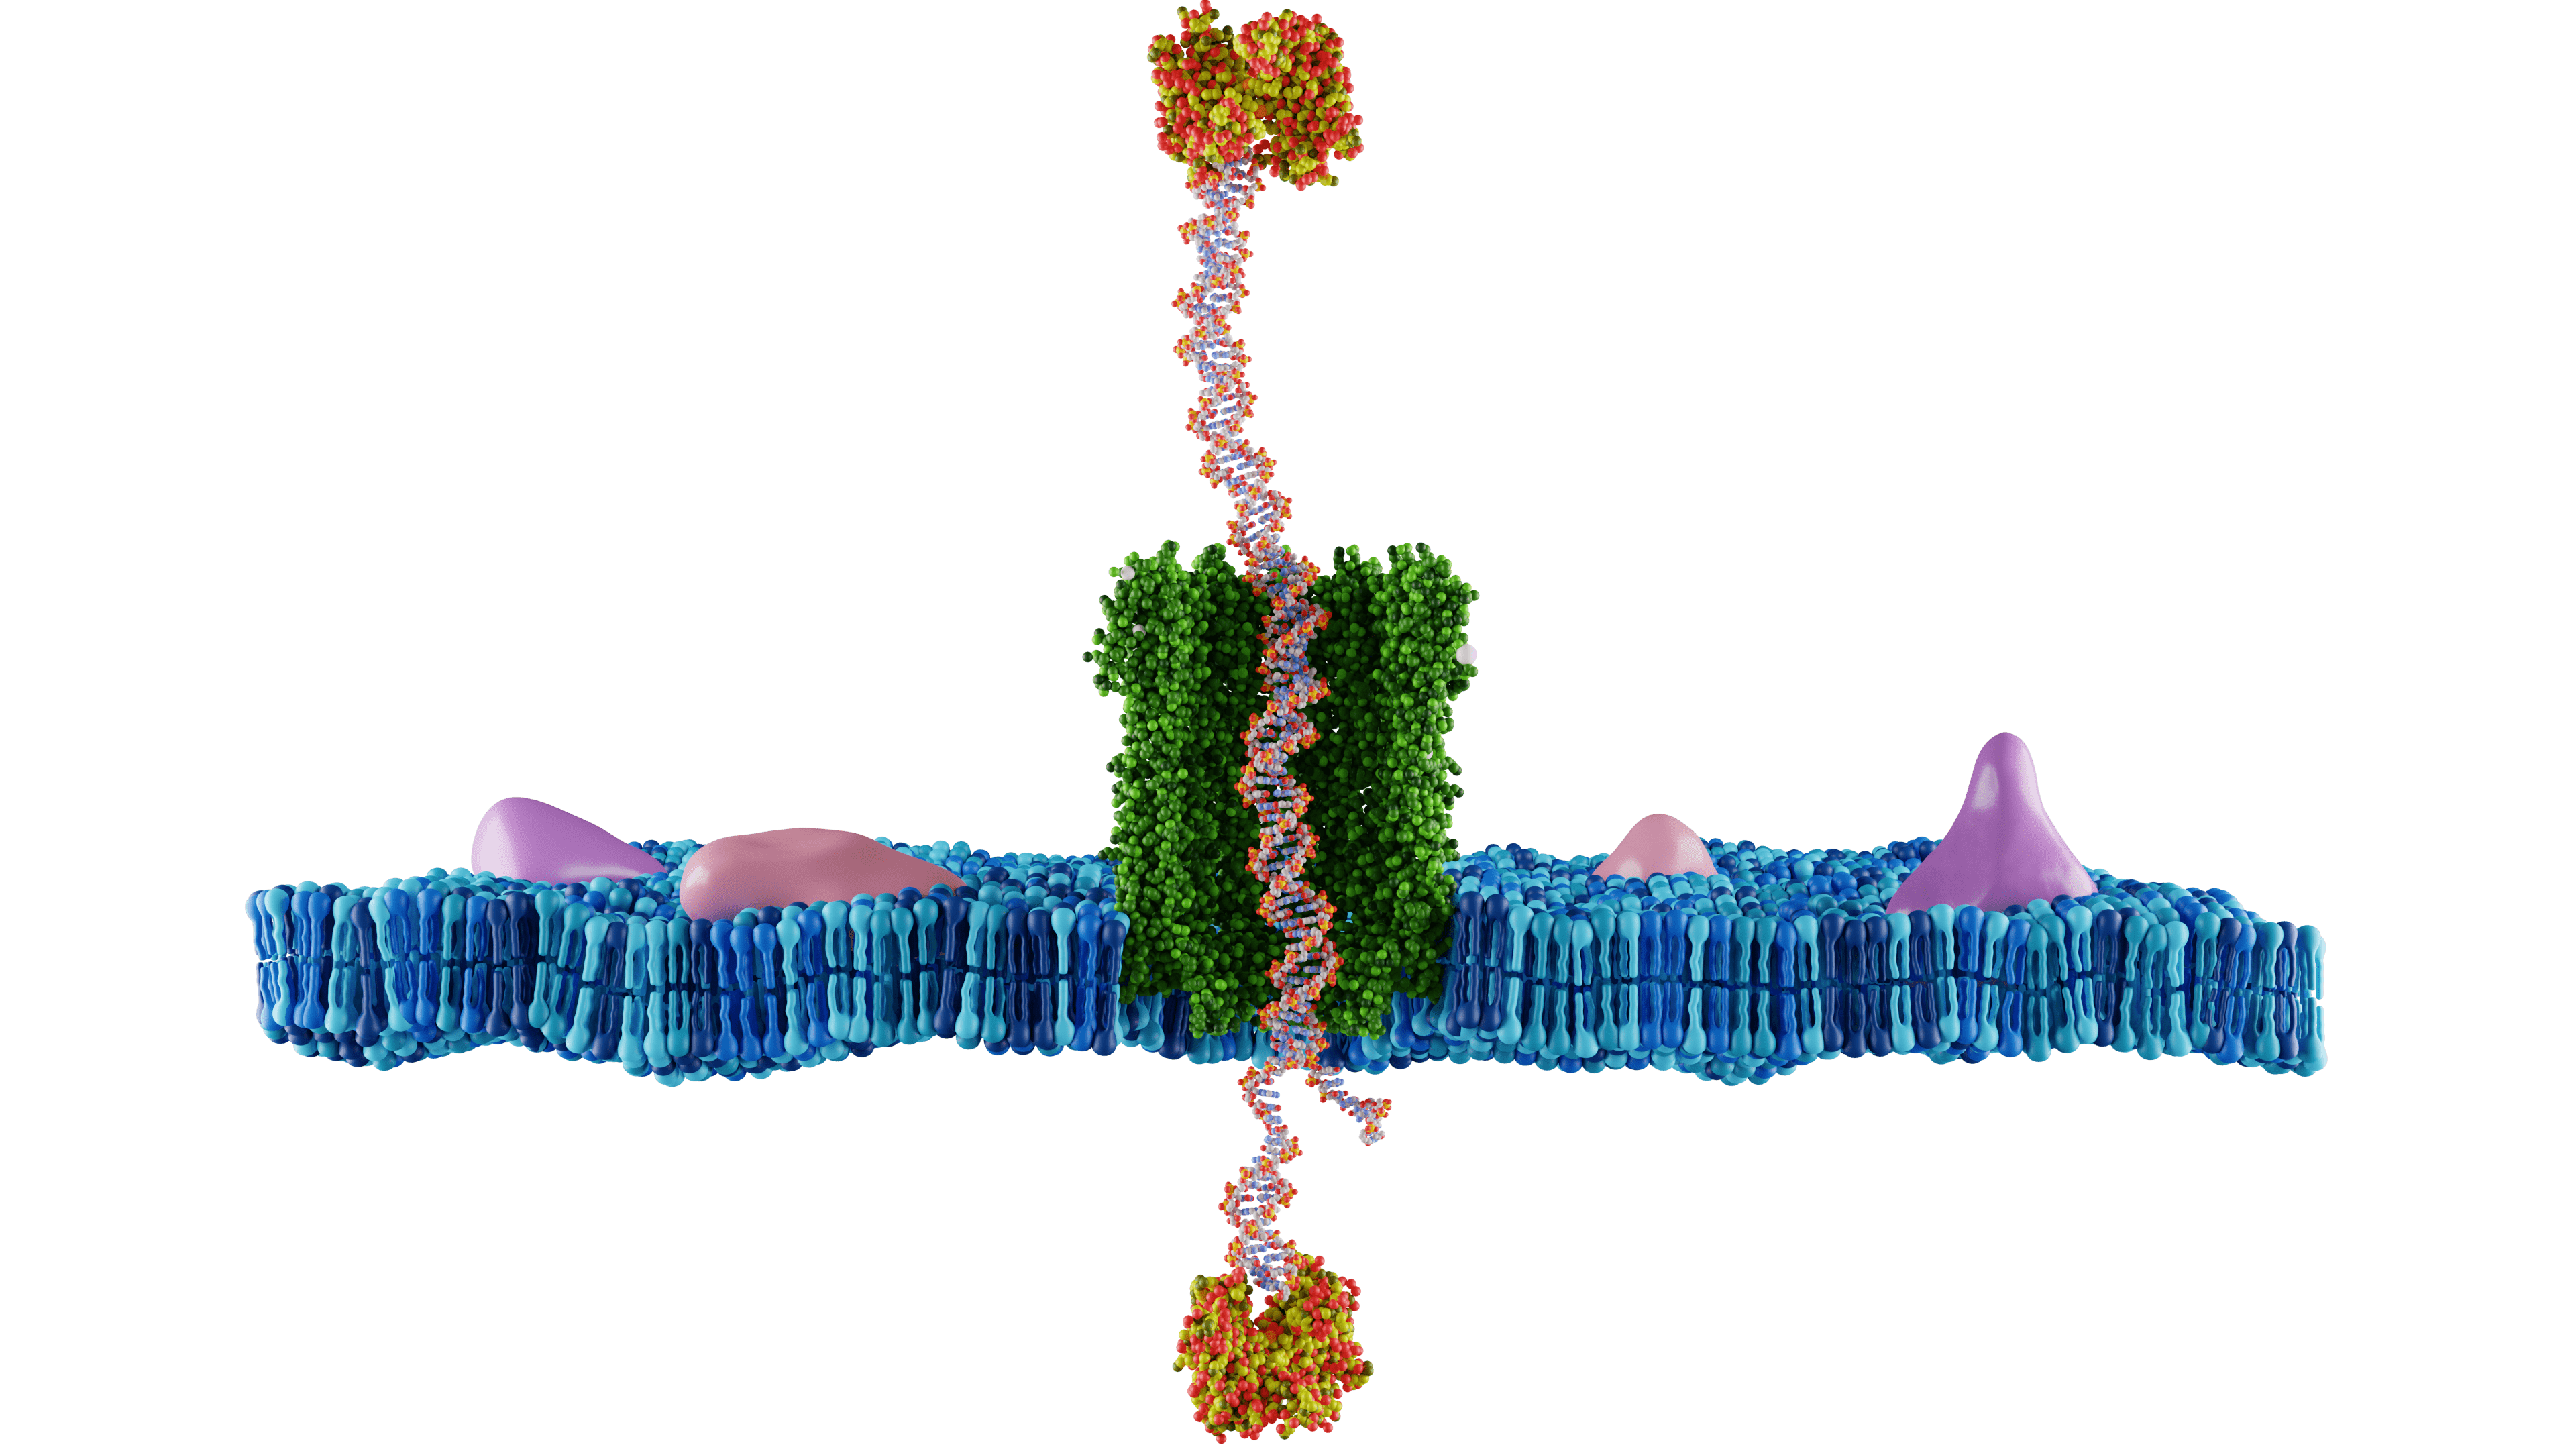
\includegraphics[height=9.5cm, width = 15.5cm]{Figures/CoverPhoto.png}
\vspace*{5cm}
\begin{center}
    \begin{figure}[H]
        \centering
        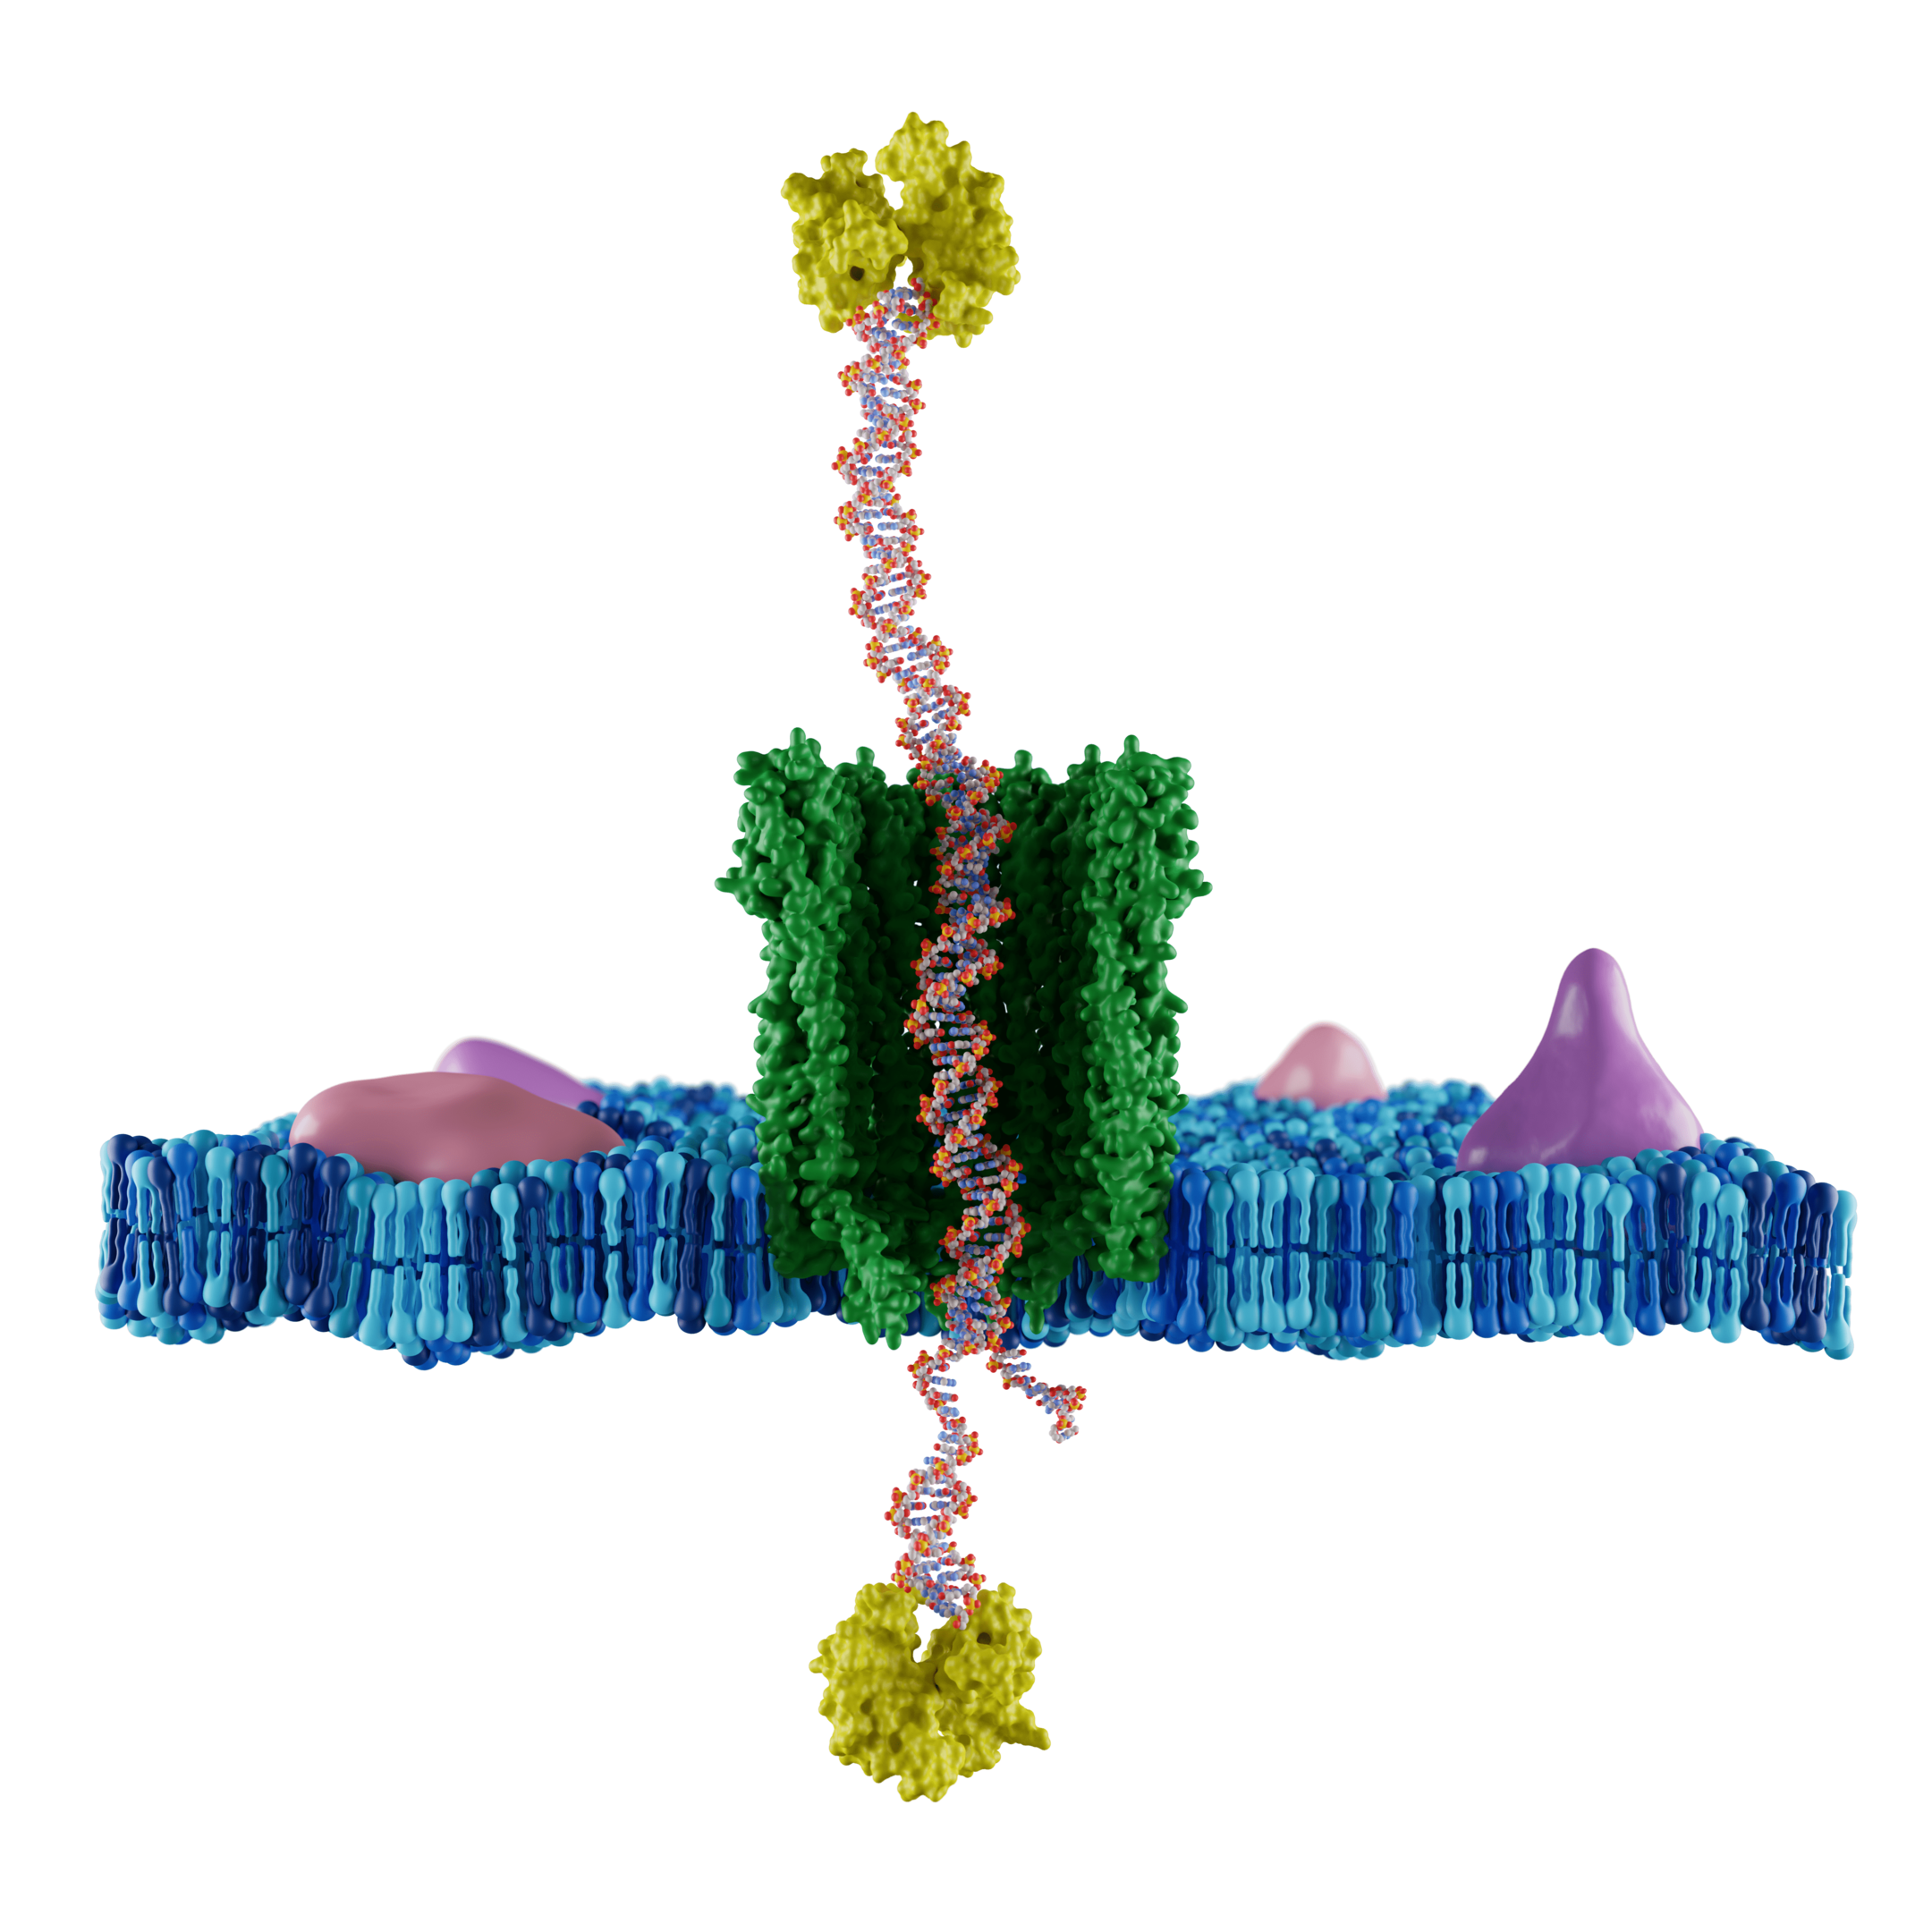
\includegraphics[scale=0.182]{Figures/Coverphoto.png}
    \end{figure}
\end{center}
%
\vfill
